\chapter{Viewpoints}
\label{chap:viewpoints}

In dit hoofdstuk worden \emph{design viewpoints} besproken die relevant zijn voor het systeem. 
Naarmate de ontwikkelingen van CalZone vorderen, zullen deze viewpoints uitgebreid worden en kunnen er view points bijkomen. 
Op het einde van de laatste iteratie wordt verwacht dat alle requirements uit het SRS van dit project ontworpen zijn. 
Voorlopig wordt er in de volgende secties enkel het design besproken van de eerste en tweede iteratie.

\section{Context}
\label{sec:context}

De gebruikers van het systeem zijn onder te verdelen in 5 categori\"{e}n: externen, studenten, professoren, assistenten en programmabeheerders. 
Elk soort gebruiker moet in de finale versie van CalZone in staat zijn de functionaliteiten die specifiek aan deze gebruikers zijn toegekend toe te passen zoals beschreven in het SRS van dit project. 
\\
Gebruikers zijn in staat om zich te registreren in het systeem. 
Hierdoor kunnen ze inloggen en bezitten deze gebruikers een profielpagina.
Daarnaast is de gebruiker in staat deze profielgegevens aan te passen.
In deze iteratie is de functionaliteit voor een algemene gebruiker uitgebreid met de mogelijkheid om lessenroosters en lokalenroosters te bezichtigen.
\\
Eveneens is er functionaliteit voorzien voor specifieke gebruikers: studenten, professoren, assistenten en administrators.
Deze uitbreidingen zijn te bezichtigen in het use case diagram in figuur \ref{fig:usecase}.

\begin{figure}[H]
	\centering
	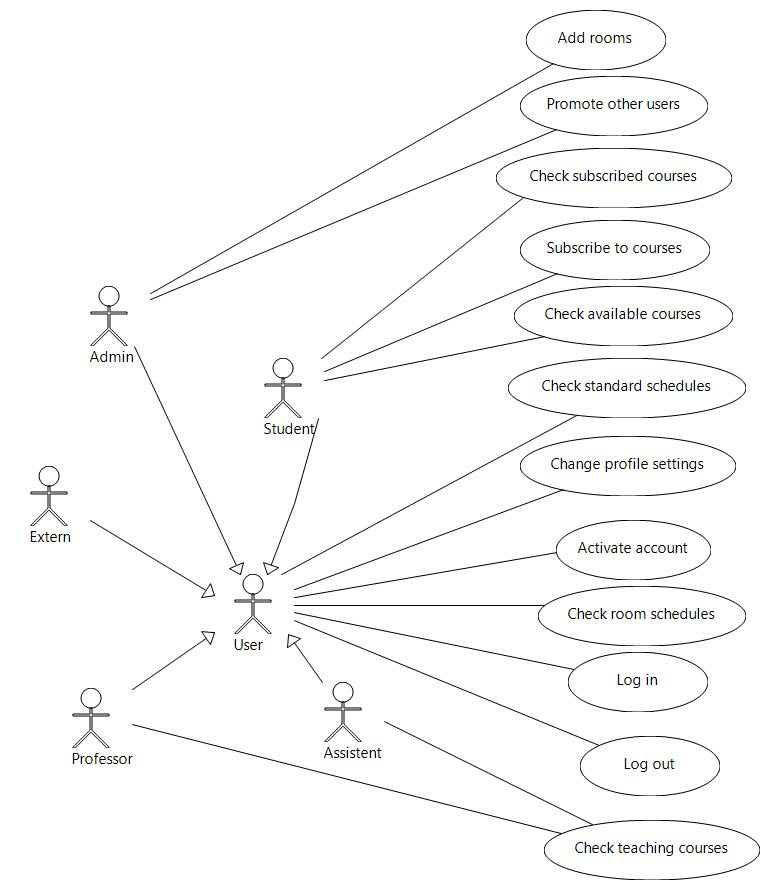
\includegraphics[scale=0.5]{img/use_cases}
	\caption{Use case diagram}
	\label{fig:usecase}
\end{figure}

\section{Logica}
\label{sec:logica}

In deze sectie worden de verschillende modules en packages behandeld die tesamen het huidige systeem vormen.

\subsection{Controllers}
\label{subsec:controllers}

Deze klassen zijn verantwoordelijk om de HTTP-requests te verwerken. 
Deze klassen zorgen dus voor een propagatie van (functionaliteits)verzoeken van de front-end naar de back-end. 
Eveneens zorgen deze klassen ook voor een propagatie van data van de back-end naar de front-end. 
Dit laatste uit zich in het voorzien van webpagina's.
Met andere woorden zorgen de controllers dus voor de mogelijke views en voorzien dus de mogelijkheid om de functionaliteiten opgesomd in het use case diagram van sectie~\ref{sec:context} uit te voeren. 
Voor volgende concepten zijn er nu controllers voorzien:

\begin{itemize}
	\item Login
	\item Profieloverzicht
	\item Registratie
	\item Accountactivatie
	\item Lokalen
	\item Vakken toevoegpagina
	\item Ingeschreven vakken pagina
	\item Email
\end{itemize}

\subsection{Databaseklassen}
\label{subsec:databaseklassen}

CalZone maakt gebruik van een relationele databank, MySQL, als back-end voor dataopslag. 
Om informatie vanuit deze databank te lezen en er naartoe te schrijven zijn er enkele klassen voorzien die een abstractie bieden voor het openen en sluiten van de connectie met de databank en het sturen van queries naar de databank. 
Volgende klassen zijn hiervoor voorzien:

\begin{itemize}
	\item DbConfig: Deze klasse voorziet de mogelijkheid om gegevens op te halen om toegang te kunnen krijgen tot een bepaalde databank. 
	Deze gegevens de gebruikersnaam, het wachtwoord en de locatie van de databank. 
	\item DbLink: Het openen en sluiten van de databankconnecties samen met het sturen van queries en het ontvangen van resultaten.
	\item DbTranslate: Een collectie van methodes die gemapt worden op queries naar de onderliggende databank
\end{itemize} 

\subsection{Data Access Objects}
\label{subsec:dao}

Het ophalen van data uit de MySQL databank gebeurt via \emph{Data Access Objects} of kortweg DAO's. 
Deze objecten gebruiken de algemene databasemethoden voorzien door de databaseklassen aangehaald in subsectie~\ref{subsec:databaseklassen} om specifieke data op te halen uit de databank en in te laden in de beschikbare klasses in het systeem. 
Ook wordt specifieke informatie via deze DAO's weggeschreven naar de databank. 
Volgende DAO's zijn aangemaakt in deze iteratie:

\begin{itemize}
	\item ActivationKeyDao: de activatiesleutels gebonden aan een geregisteerd account. 
	\item UserDao: gebruikergegevens
	\item SessionDao: gebruikerssessies met het systeem.
	\item PasswordDao: de gehashte wachtwoorden van gebruiker oproepen
	\item StudentDao: studenten ophalen uit de databank en inladen in de bestaande studentenklasse
	\item RoomDao: lokalen ophalen uit de databank en inladen in de bestaande lokalenklassen
\end{itemize}

\subsection{Validators}
\label{subsec:validators}

Binnenin het systeem dient sommige data gecontroleerd te worden op geldigheid. 
Deze validatorklassen zijn verantwoordelijk om geldigheid van bepaalde informatie te controleren en aan te geven indien deze info niet geldig is. 
Volgende validators zijn in het huidige systeem aanwezig:

\begin{itemize}
	\item Email: controle op het emailadres
	\item Gebruikers: controle op de gebruikersnaam om profiel
	\item Lokalen
\end{itemize}
\section{Data}
\label{sec:data}
De evolutie die het design in deze iteratie heeft ondervonden is vooral te merken in de database.
Het datamodel is uitgebreid opdat de databank in staat is om vakken, lokalen en allerhande concepten omtrend deze vakken en lokalen op te kunnen slaan. Deze concepten zullen laterinvloed hebben op het plannen van de lessenroosters en lokalenroosters via de scheduler.\\

Ook werden aanpassingen uitgevoerd aan het user management zodat bij implementatie gebruik gemaakt kon worden van de module Spring Security\cite{spring-security} om de authenticatie van gebruikers af te handelen.\\

Figuur~\ref{fig:EER diagram} toont het EER-model van de databank. Om overzicht te bewaren worden de attributen die iedere entiteit bezit niet weergegeven in dit model.

\begin{figure}[H]
	\centering
	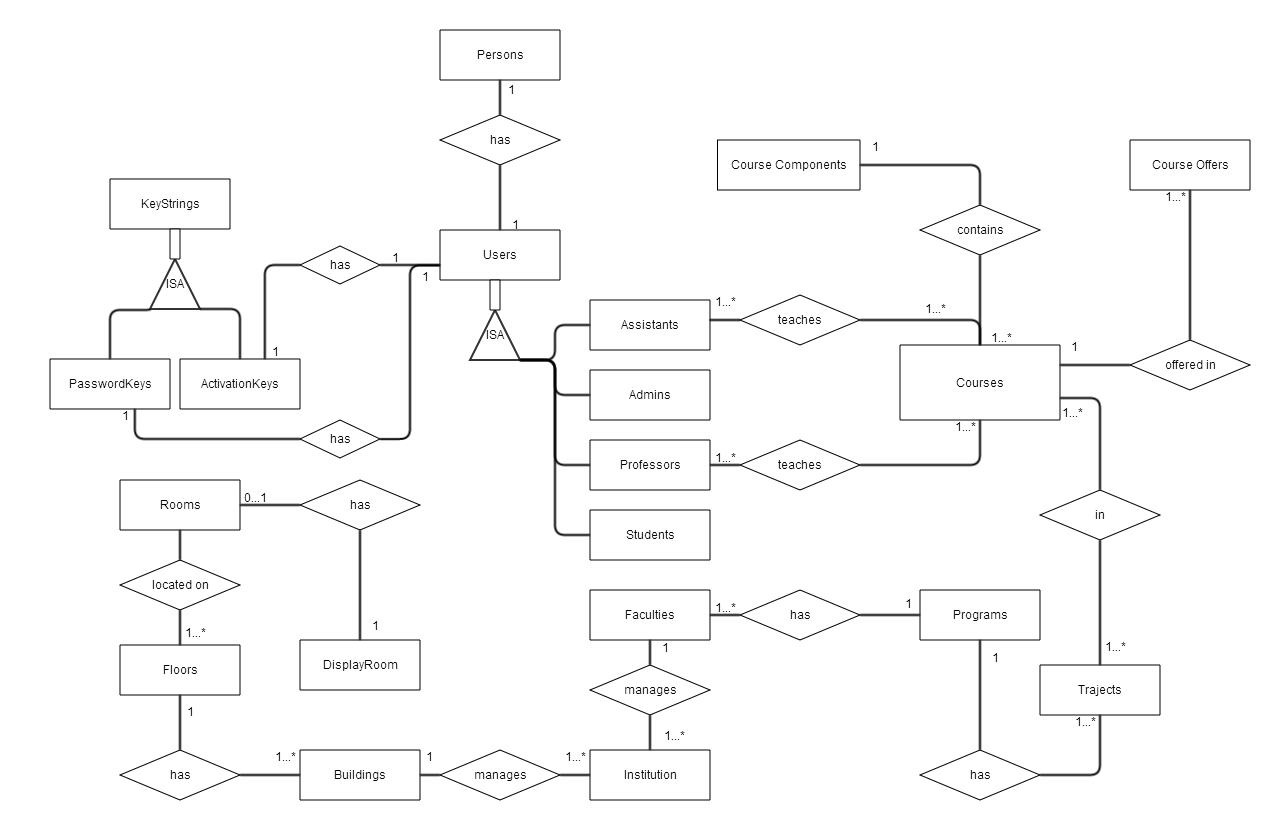
\includegraphics[scale=0.4]{img/ER2-gliffy}
	\caption{EER diagram}
	\label{fig:EER diagram}
\end{figure}

\section{Structuur}
\subsection{Leslokalen en vakken}
Volgend UML diagram beschrijft de structuur van de verscheidene klassen betreffende leslokalen en lessen die met elkaar gerelateerd zijn op het logisch niveau van het systeem.
Deze klassen bezitten data vanuit de databank die nodig zullen zijn om lessenroosters en examenroosters te plannen.

\begin{figure}[H]
	\centering
	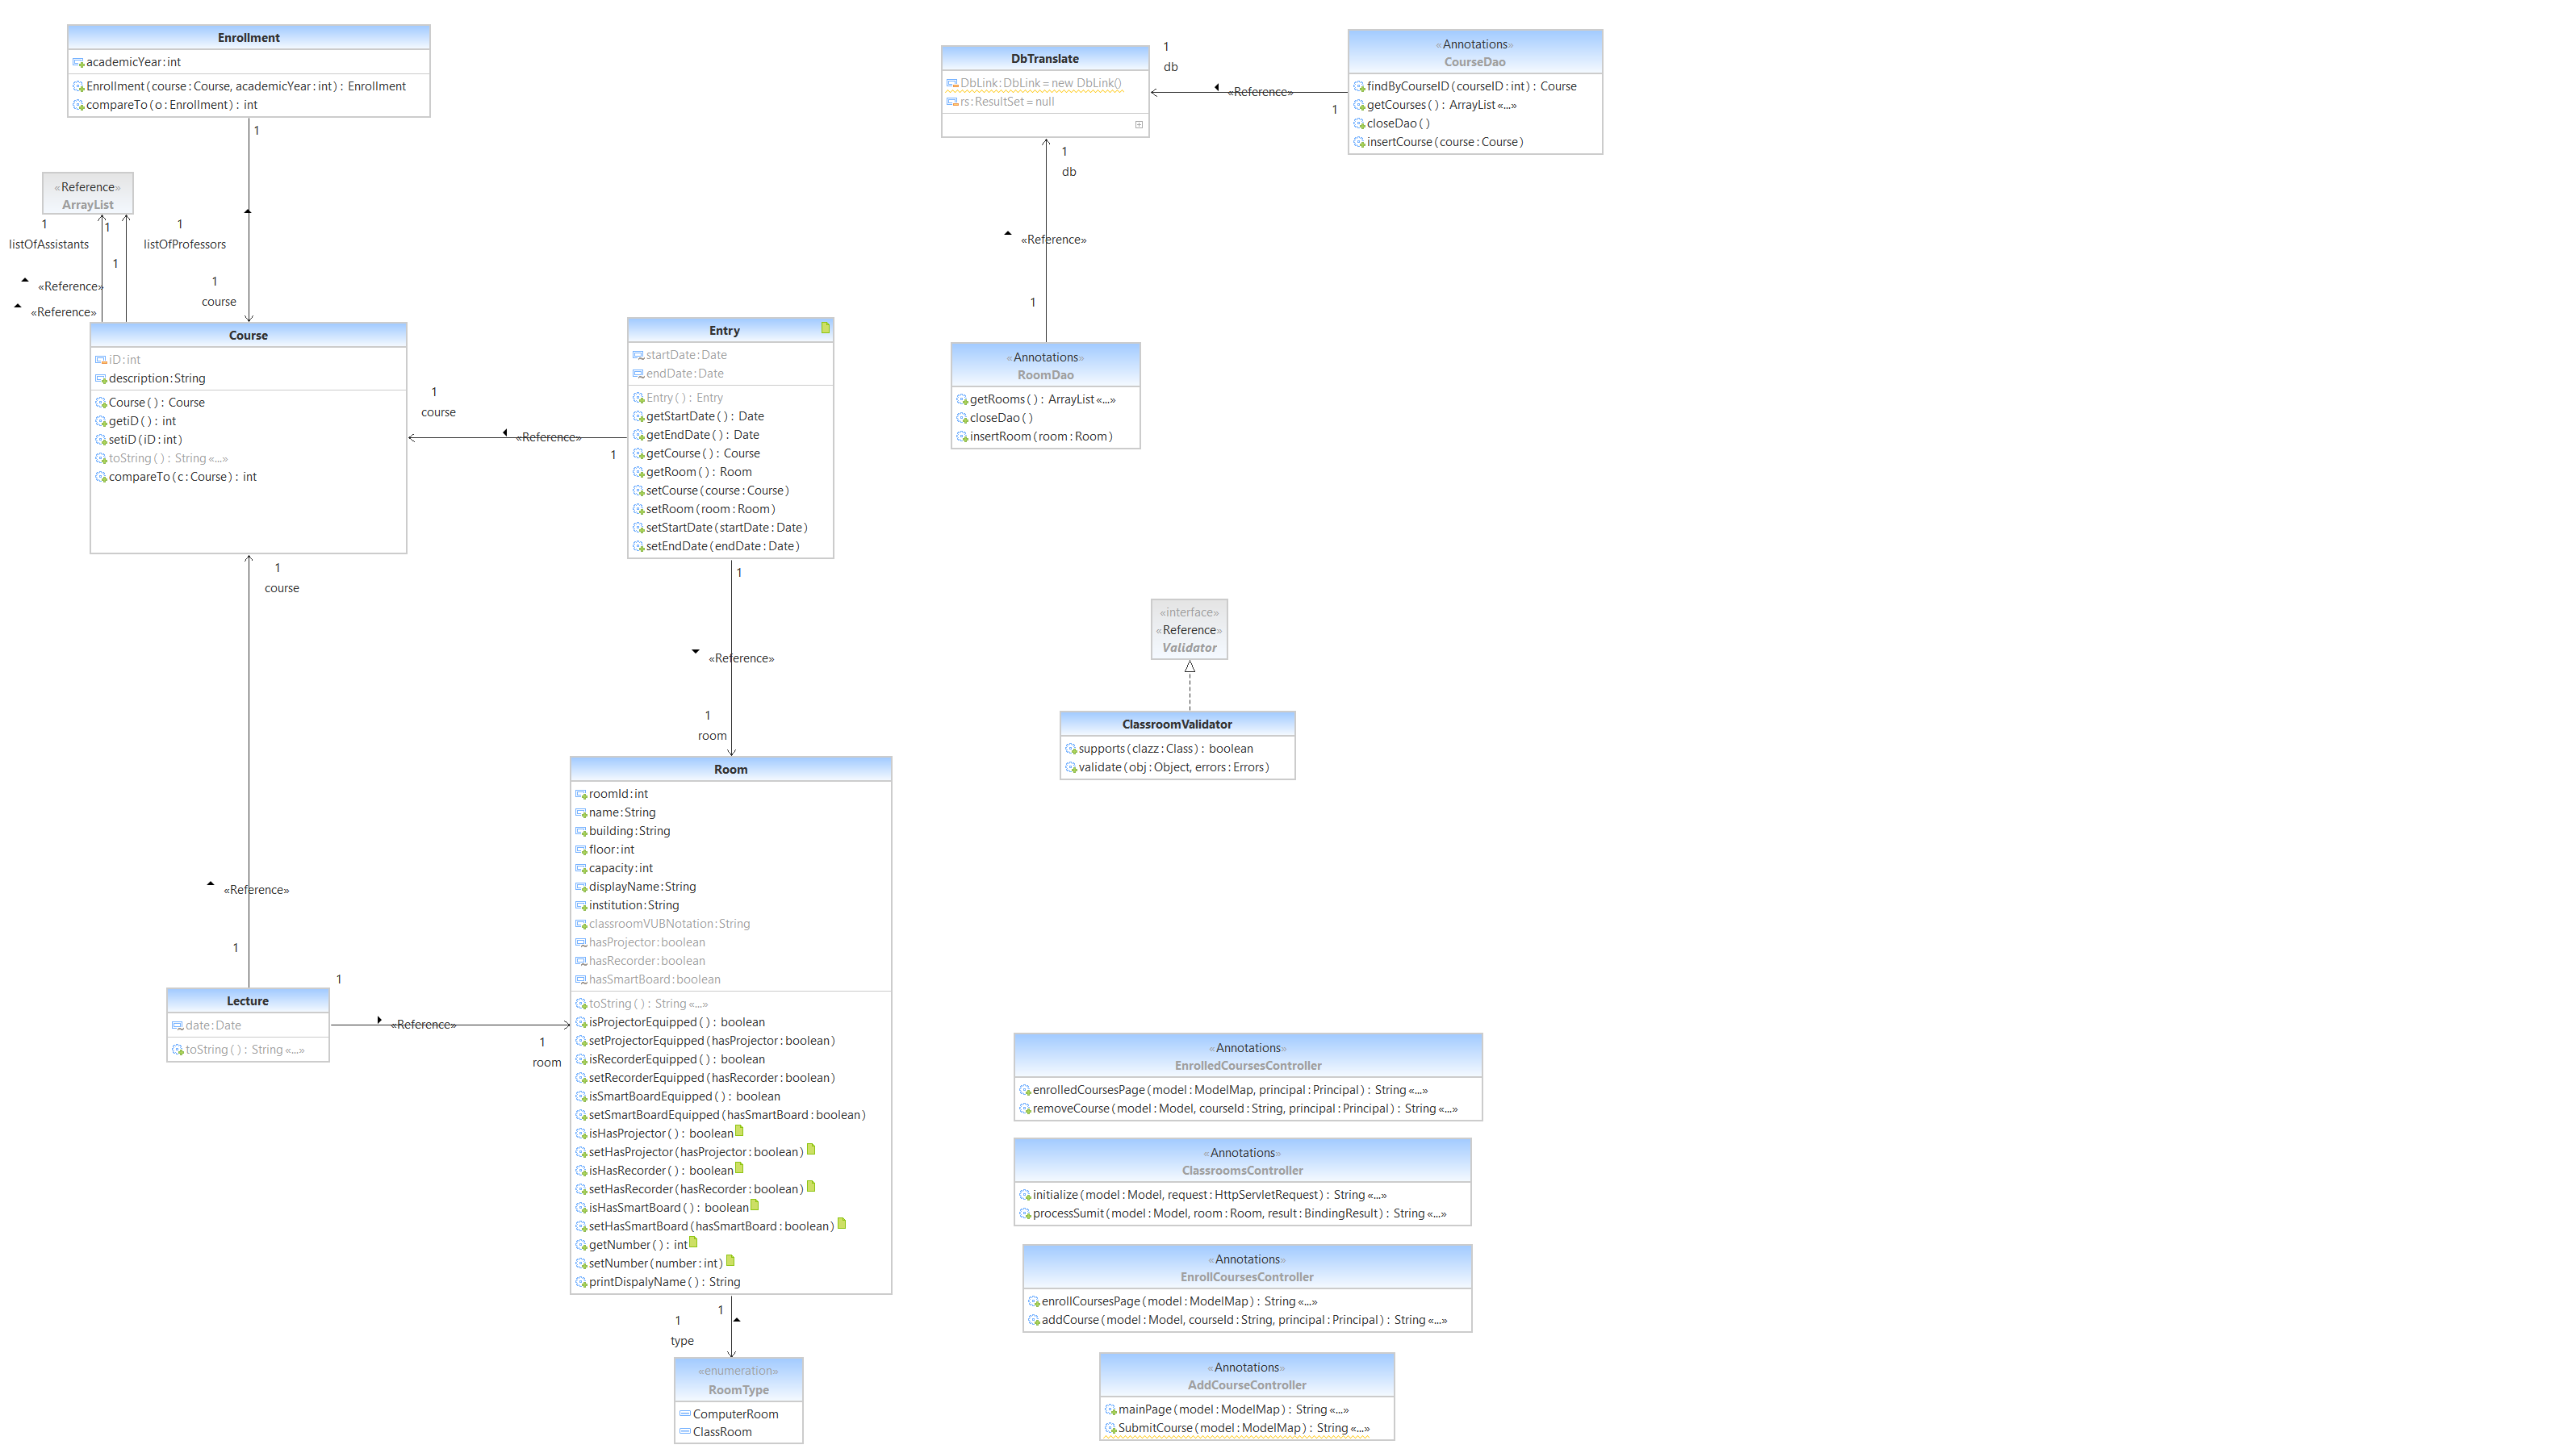
\includegraphics[scale=0.2]{img/roomsAndCourses}
	\caption{UML klassediagram voor leslokalen en vakken}
	\label{fig:roomsAndCourses}
\end{figure}

\section{Algoritmes}
\subsection{Scheduling}
Het huidige plan is om gebruik te maken van de Java Library 'Optaplanner'